\chapter{実験2}

\section{目的}

    実験2では、実験1で使用した刺激を元にした単色パッチを用いて明るさを定量化する。
    実験1の光沢感の色度による傾向と明るさの色度による傾向を比較することで、光沢感と明るさの相関を明らかにする。


\section{実験方法}
    \subsection{実験環境、被験者}

        実験2で用いた装置と参加した被験者は、いずれも実験1と同一であった。

    \subsection{実験刺激}

        \begin{figure}[h]
            \centering
            
\includegraphics[width=14.0cm]{./img/ex2_stimuli2.png}
            \caption{1試行に呈示される実験刺激の例}
            \label{ex1_procedure}
        \end{figure}

        \begin{figure}[h]
            \centering
            
\includegraphics[width=14.0cm]{./img/patchStimuli.png}
            \caption{参照刺激として使われた色}
            \label{ex1_procedure}
        \end{figure}

        図に実験2で使用する刺激と、参照刺激に使われた色を示す。
        参照刺激として使われた18種類の色度は、実験1で用いたStanford DragonのSD着色条件、D着色条件のそれぞれの刺激の平均色(以下SD平均,D平均とする)である。

    \subsection{実験手続き}

        実験2では調整法によりカラーパッチの知覚的な明るさを計測する。
        実験2の1試行の流れを図に示す。
        各試行では、はじめに黒背景のみからなるブランク画面が 1000 ms の間呈示された。
        次に参照刺激であるカラーパッチとテスト刺激である無彩色パッチからなる刺激対が呈示された。
        被験者はトラックボールを左右に回すことにより、無彩色パッチの輝度を調節し, カラーパッチと同じ明るさに知覚されるようになるまで操作した。
        同じ明るさと判断した場合はトラックボールマウスの右クリックを押すことで次の試行のブランク画面へ移行した。
        この時、テスト刺激の輝度が記録された。
        カラーパッチと無彩色パッチの左右位置は試行ごとにランダムに決定された。
         
        各セッションは 2 着色条件 ✕ 色度 9 通り = 18 試行からなり、各被験者は全体で5セッションの実験を行った。
        各セッションの 18 試行で使われる参照刺激は全てランダムな順序で選ばれた.

\section{実験結果}

    \begin{figure}[h]
        \centering
        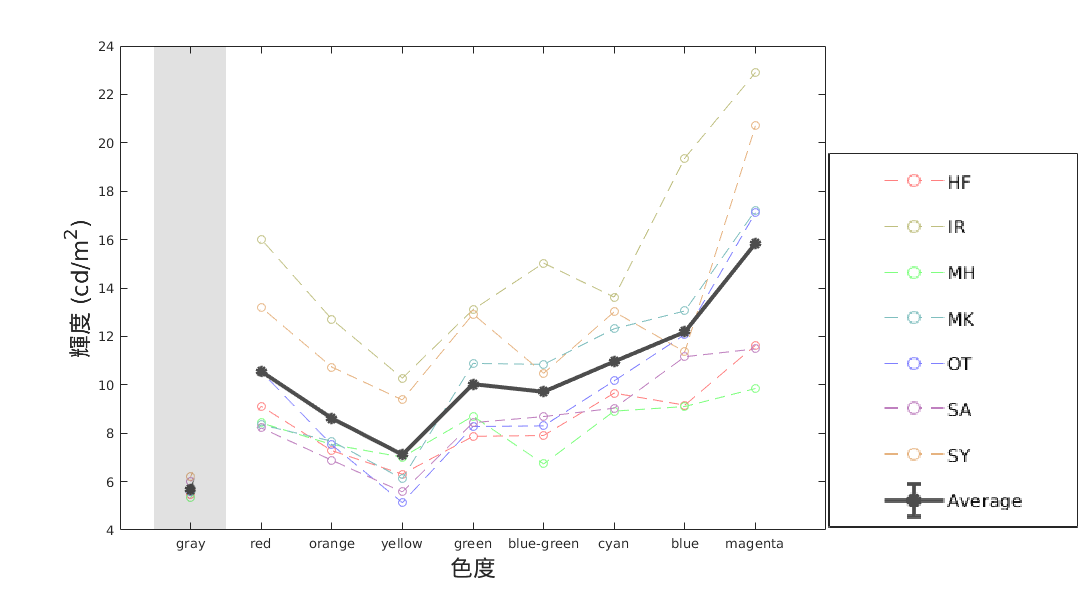
\includegraphics[width=14.0cm]{./img/ex2_res_SD_p.png}
        \caption{SD平均条件におけるテスト刺激の輝度}
        \label{ex2_SD}
    \end{figure}

    \begin{figure}[h]
        \centering
        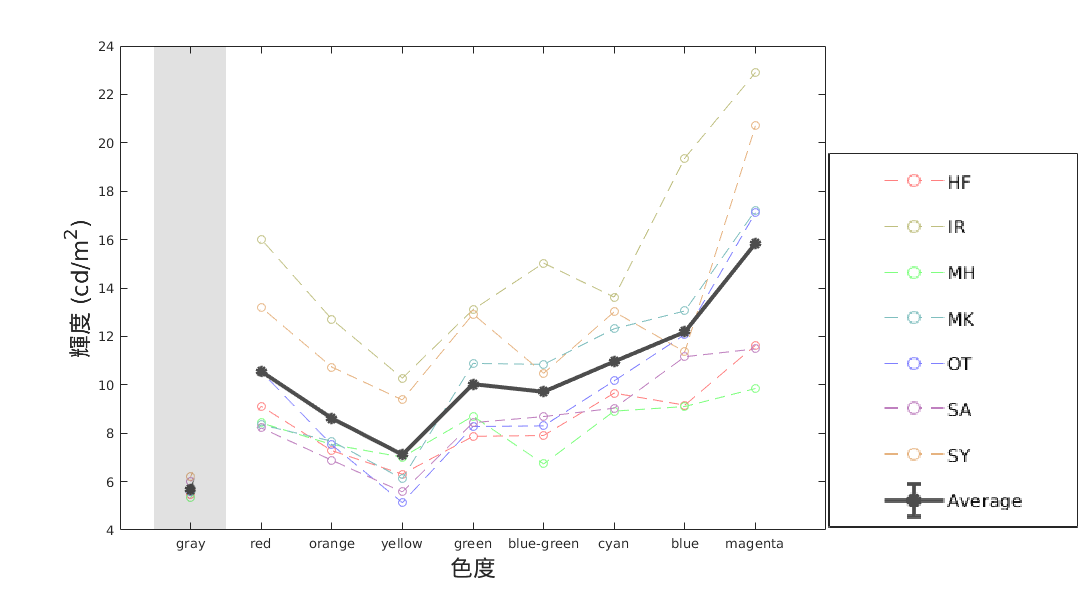
\includegraphics[width=14.0cm]{./img/ex2_res_SD_p.png}
        \caption{D平均条件におけるテスト刺激の輝度}
        \label{ex2_D}
    \end{figure}

    SD平均、D平均ともに同様の傾向が得られた。
    この結果と実験1の結果から、光沢感と明るさの相関を調べる。

    尺度を揃えるため、実験1と実験2のデータの両方に正規化を行い、条件ごとに散布図にプロットした。
    各点の色は実験で使われた9種類の色度からなり、ある点の色の色度条件について横軸は明るさを、縦軸は光沢感を表している。
    また表は各物体形状・着色条件における相関係数を表す。

    \begin{figure}[h]
        \centering
        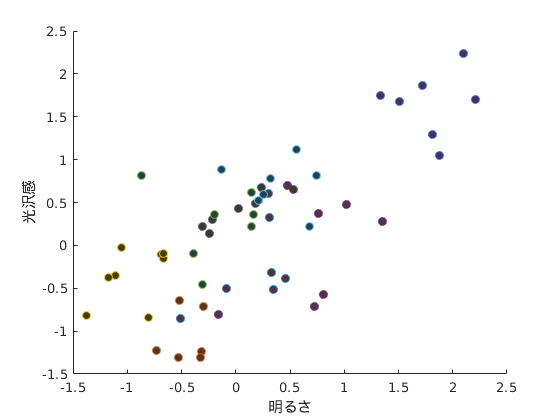
\includegraphics[width=12.0cm]{./img/ex3_DSD.png}
        \caption{Dragon:SD}
        \label{ex3_DSD}
    \end{figure}

    \begin{figure}[h]
        \centering
        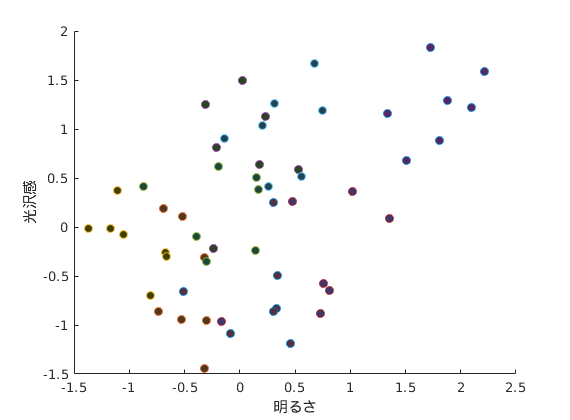
\includegraphics[width=12.0cm]{./img/ex3_BSD.png}
        \caption{Bunny:SD}
        \label{ex3_DSD}
    \end{figure}

    \begin{figure}[h]
        \centering
        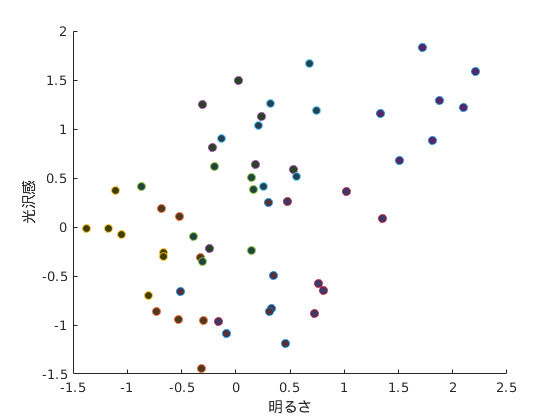
\includegraphics[width=12.0cm]{./img/ex3_DD.png}
        \caption{Dragon:D}
        \label{ex3_DD}
    \end{figure}

    \begin{figure}[h]
        \centering
        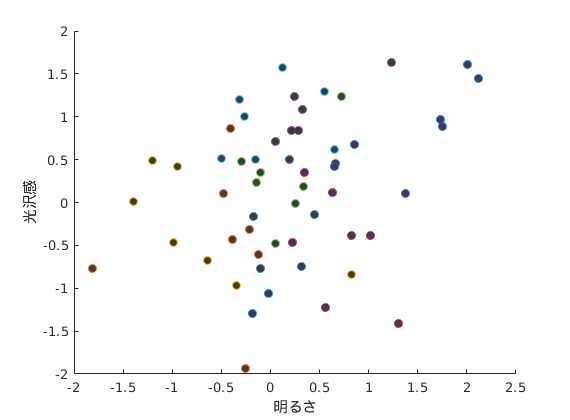
\includegraphics[width=12.0cm]{./img/ex3_BD.png}
        \caption{Bunny:D}
        \label{ex3_BD}
    \end{figure}

    \begin{table}[h]
        \centering
        \caption{各条件の相関係数}
        \begin{tabular}{|l||c|c|} \hline
                        & SD       & D        \\ \hline \hline
            Dragon      & 0.8828   & 0.8290   \\ \hline
            Bunny       & 0.6490   & 0.5184   \\ \hline
        \end{tabular}
    \end{table}

    Dragon:SD、Dragon:Dにおいて比較的強い正の相関が見られたが、これに比べてBunny:SD,Bunny:Dの相関係数は小さい値を示した。
    この結果は、H-K効果がもたらす知覚的な明るさは光沢感に寄与する要因の一つであるが、他の要因も寄与している可能性を示唆する。